\section{Utterance cost predicts intensifier strength}

The proposal detailed above predicts an association between measures of cost and strength of interpretations.
In our first series of studies, detailed in this section, we tested whether our measures of communicative cost can in fact predict intensifier strength.%
% \footnote{
% Demos for all studies can be found at
% \url{http://cocolab.stanford.edu/links_for_papers/bennett2017extremely/demos/}
% }

We used two measures of intensifier strength.
Our first measure of intensifier strength (used in Studies \hyperref[sec:study1a]{1a} and \hyperref[sec:study1b]{1b}) was asking participants for a numeric interpretation of intensified adjective phrases.
Our second measure (used in Study \hyperref[sec:study2]{2}) was asking participants to rank the strength of adjective phrases that differed only in their intensifier.
The first measure allowed us to compare our full set of intensifiers to one another on a numeric scale.
The second allowed us to test our hypothesis on a wider range of adjectives at once, some of which (e.g. \w{beautiful}) correspond to more abstract, non-numeric scales.

\subsection{Study 1a \label{sec:study1a}}

In Study \hyperref[sec:study1a]{1a}, we tested the qualitative prediction that as the communicative cost of an intensifier increases, so will the numeric interpretation of the adjective phrase it is part of.
We tested this prediction by eliciting free-response price estimates from participants for phrases such as \w{very expensive watch} and determining whether the prices participants responded with were correlated with independent measures of communicative cost.

\subsubsection{Methods}

\paragraph{Participants}

30 participants with US IP addresses were recruited through Amazon’s Mechanical Turk and paid \$0.40 for their participation. 1 participant was excluded from the analysis for admitting that they did not think they followed the instructions in a post-experiment survey and another for not being a native speaker of English.

\paragraph{Items}

The sentences in the study included intensifiers paired with the adjective \w{expensive} (Figure \ref{fig:question_study1a}).
There were three categories of objects (\w{laptop}, \w{watch}, and \w{coffee maker}) and 40 intensifiers (see Table \ref{table:intensifiers_study1a}).

The intensifiers in our study were collected from word lists online and searching thesauri for more intensifiers.
We chose intensifiers that have a wide range of frequencies and excluded intensifiers that are either more commonly used to signal affect than to signal degree (e.g. \w{depressingly expensive} might indicate a degree, but it mainly indicates affect) or are ambiguous between other parts of speech (e.g. \w{super} can be used as an intensifier, as in ``super expensive'', but it can also be used as an exclamation, as in ``Super!'').

We chose the domain of price for Study \hyperref[sec:study1a]{1a} and used only the adjective \w{expensive}.
Because price constitutes a quantitative scale with standard units (dollars for our US participants), this allowed us to quantitatively measure the relative strengths of different intensifiers.

\paragraph{Procedure%\footnote{A demo of Study \hyperref[sec:study1a]{1a} can be found at \url{http://cocolab.stanford.edu/links_for_papers/bennett2017extremely/experiments/Study1a/.}}}
}

We asked participants to estimate the prices of different objects based on different descriptions of those objects. 

Each participant gave price judgments for every intensifier-category pairing in a randomized order (different for different participants), for a total of 120 price judgments per participant.  

The only allowable characters in responses were the digits 0-9 and (optionally) one decimal point (.) followed by two digits. All other responses were immediately rejected.
Participants were prevented from continuing until they provided a valid numeric response for each trial.

\begin{figure}[ht]
\begin{center}
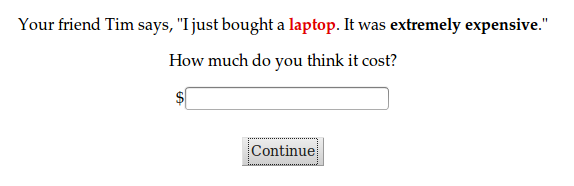
\includegraphics[width=0.4\textwidth]{exp1-q.png}
\end{center}
\caption{Screenshot from Study \hyperref[sec:study1a]{1a} target question.} 
\label{fig:question_study1a}
\end{figure}

\subsubsection{Corpus Methods}

Table~\ref{table:intensifiers_study1a} shows word frequency and length in syllables for the intensifiers used in Study \hyperref[sec:study1a]{1a}.
The frequencies were collected from the Google Web 1T 5-grams database \cite{brants_web_2006}.\footnote{
  We also ran the same analyses on frequency information collected from the Google Books American Ngrams Corpus \cite{michel_quantitative_2011} and found similar results.
}
In the analysis below we use word length and word surprisal (negative log-frequency) as proxies for a word's cost, as motivated above.
The syllable lengths of our intensifiers and the surprisals were correlated ($r = 0.26$).
This correlation makes it somewhat difficult to determine the effect of one measure of cost above and beyond the other.
In our first series of studies, we focus on the primary effect of surprisal, since we have more range in surprisal across intensifiers than in length and since we manipulate length in syllables for our next series of studies.
However, we model both measures of communicative cost in our analyses: We include both predictors in regressions and report likelihood-ratio tests between the full model and simpler models.

\subsubsection{Analysis}

Prices that participants give obviously vary systematically with the object (expensive laptops tend to be more expensive than expensive coffee makers).
Responses are also likely sensitive to variation across participants due to their different beliefs about likely prices.
Because we have few objects, we are unable to model the variation due to object, but because we have many intensifiers (they are fully crossed with objects), normalizing is fairly effective at converting all objects to the same scale.
We are not theoretically interested in the variation due to objects, and so in order to compare intensifiers across these objects, we first normalized log-transformed prices within participant and object.
We used the logarithm of participants' price estimates because of evidence that people's representation of numbers, including prices, is logarithmic \cite{fechner_elements_1860}.\footnote{
  I.e. the perceptual distance between two prices the same dollar amount apart is more for small numbers (e.g. \$3 and \$6) and less for large numbers (e.g. \$1,543 and \$1,546).
}

We ran a linear mixed effects regression to predict scaled price estimates. We included centered fixed effects of length and surprisal. To model random effects due to participant, we only included random slopes, since the normalization gives each participant an intercept of 0.  We also included a random intercept for intensifier to model any idiosyncratic meaning there might be to a particular intensifier beyond communicative cost. 
The predicted mean $y_{ij}$ for the $i^{th}$ intensifier and the $j^{th}$ participant under this model is shown in Equation \ref{eq:study1}, where $f_i$ represents the surprisal of the $i^{th}$ intensifier and $l_i$ represents its length. %with random by-intensifier intercepts $I_i$ and random by-participant slopes $P_{1j}$ and $P_{2j}$.


\begin{equation}
\label{eq:study1}
y_{ij} = \beta_0 + {U_0}_{i} + ({U_1}_{j} + \beta_1) {f}_{i} + ({U_2}_{j} + \beta_2) {l}_{i}
\end{equation}

As previously noted, surprisal and length in syllables are correlated in this set of intensifiers ($r=0.26$).
We focus on surprisal as our primary effect, but we are also interested in the independent contribution of length in syllables.
To address the independent effects of these variables, we ran model comparisons using log likelihood, leaving out information about one of the predictors.
We also ran two additional mixed effects reggressions: one in which the suprisal is first residualized against syllables (using ordinary linear regression), and one where length is residualized against surprisal.

\subsubsection{Results}

If the meaning of an intensifier is stronger for higher cost intensifiers, we would expect to find that as surprisal increases and length in syllables increases, the prices participants give will also increase. 
We find that this is the case for surprisal, but do not show a significant effect of syllable length beyond the effect of surprisal.
Our results are shown in Figure~\ref{fig:plot_study1a}, in a way that highlights the surprisal predictor.
\eb{We present full regression output in Appendix B.}

We find a significant effect of surprisal ($b=0.106,t(38.9)=3.411,p=0.0015$) such that less frequent words tend to be associated with higher price estimates.
In this regression, we did not a significant effect of syllable length ($p=0.0936$), above and beyond surprisal.

Because surprisal and syllable-length are correlated, in addition to the analysis reported here we also used likelihood ratio tests to compare the full model to models with only one of the two predictors.
These tests show that length in syllables alone account for the data less well than the full model ($\chi^2(8)=17.055, p<0.0005$) and that surprisal alone also accounts for the data less well than the full model ($\chi^2(8)=13.697, p<0.0005$), suggesting that both might separately contribute to the cost of the utterance.
When length was residualized with respect to suprisal, both the residuals ($b=0.106,t(38.9)=3.411,p=0.002$) and length ($b=0.202,t(40.9)=2.693,p=0.010$) were significant predictors of scaled ratings. However, when surprisal was residualized with respect to length, surprisal ($b=0.12, t(39.9)=3.985, p<0.0005$) but not the residuals ($p=0.0936$) was a significant predictor of scaled ratings. This discrepency is likely a due to the fact that, since length in syllables is a discrete value taking one of 6 values, whereas surprisal is continuous, length can be more informatively predicted from surprisal (different surprisals can map onto approximately the same length) than surprisal can be predicted from length (the same length cannot map onto different surprisals).

Overall, we confirmed our main prediction that intensifiers that are less frequent (and therefore are more costly to communicate) also tend to be interpreted as having stronger meanings, at least when used to modify the adjective \emph{expensive}.
We found inconclusive results for our secondary prediction that length (another factor in communicative cost) has any effect beyond that of surprisal.
This ambiguity motivated a more sensitive dependent measure in Studies 2 and 4.

\begin{figure}[ht]
\begin{center}
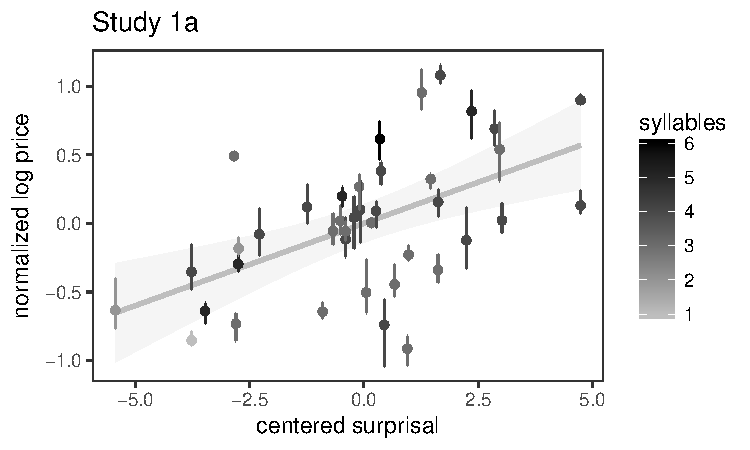
\includegraphics[width=0.5\textwidth]{images/plot_study1a.pdf}
\end{center}
\caption{Results of Study \hyperref[sec:study1a]{1a}. As surprisal increases, participants' scaled free response prices increase.} 
\label{fig:plot_study1a}
\end{figure}

\subsection{Study 1b \label{sec:study1b}}

Our initial selection of intensifiers was somewhat haphazard, being chosen partly to give the best (intuitive) chance of observing an effect. 
To show that there was no implicit bias induced by this selection, we next replicated using a revised, and more systematic, set of intensifiers.
We additionally took this opportunity to increase the sample size, guided by a power analysis based on the results of Study \hyperref[sec:study1a]{1a}.

\subsubsection{Methods}

\paragraph{Participants}

We wanted enough participants for a power level of 0.8 for the principal effect of surprisal.
Power analyses for mixed effects models with continuous predictors are not analytically straightforward, and so we approximated the number of participants necessary for our desired power by bootstrapping.
We used the data from our original Study \hyperref[sec:study1a]{1a} to simulate alternative possible datasets with different numbers of intensifiers and participants.
For each of 100 iterations, we sampled with replacement from Study \hyperref[sec:study1a]{1a} a set of $P$ participants and a set of $I$ intensifiers, varying $P$ and $I$.
We created a resampled dataset where we combined the resampled participants with the resampled intensifiers and collected the corresponding responses for each pair.
For each resampled dataset, we ran the regression model from Study \hyperref[sec:study1a]{1a}.
We computed the proportion of runs in which the surprisal term was significant and interpreted this as the power of such a study.

We found that our original Study \hyperref[sec:study1a]{1a} was somewhat underpowered by this metric (statistical power was near 0.70 for the surprisal regressor, our principal effect of interest).
For the replication, we determined that with the 71 intensifiers we collected from grammars of English (described below), 50 was the minimum number of subjects for power at the 0.8 level for the surprisal term.
We doubled this amount for a goal of 100 participants for the replication.
(Despite having sufficient power for the surprisal term, our bootstrapped power analysis suggested that even with 100 participants, the power for the length term in the model is only 0.29. We address this instead, with a direct manipulation of length, in experiments 4 and 5.)
Due to a slight error in data collection, we actually recruited 108 participants.

Following this power analysis, 108 participants with US IP addresses were recruited through Amazon’s Mechanical Turk and paid \$1.00 for their participation. 1 participant was excluded from the analysis for admitting that they did not think they followed the instructions in a post-experiment survey.

\paragraph{Items}

For Study \hyperref[sec:study1b]{1b}, we again used \w{expensive} as the adjective for the intensifiers to modify, and we again collected responses as prices in dollars.
We used the same objects (\w{laptop}, \w{watch}, and \w{coffee maker}) as in Study  \hyperref[sec:study1a]{1a}.

As we explain above, in Study \hyperref[sec:study1a]{1a} and the remaining studies detailed in this paper, our choice of the set of intensifiers to include was somewhat arbitrary and collected after formation of our hypothesis.
To address the concern that this might bias our results, we followed a more systematic procedure for generating a list of intensifiers for our replication Study \hyperref[sec:study1b]{1b}.
We sought out English grammars that listed intensifiers.
Since no single source contained the number of intensifiers desired for sufficient power in Study \hyperref[sec:study1b]{1b}, our process for collecting intensifiers in this replication was to combine word lists from multiple grammars of English.
We first found 12 grammars of English that mentioned one of the following terms: ``intensifiers'', ``adverbs of degree'', or ``amplifiers'' \cite{aarts_oxford_2014,douglas_longman_2000,declerck_comprehensive_1991,garner_chicago_2016,givon_english_1993,greenbaum_oxford_1996,huddleston_cambridge_2002,huddleston_introduction_1984,nelson_english:_2010,quirk_grammar_1972,quirk_students_1990,van_gelderen_introduction_2010}.
Most of these grammars mentioned examples of such words, and many contained lists of them.
The average length of such a list or collection was approximately 21 words.
We collected an aggregate list of all words that occurred in an ``intensifiers'', ``adverbs of degree'' or ``amplifiers'' list in at least one grammar.
Some ``downtoners''/``diminishers'' were mixed into some of these lists (e.g. \w{slightly}, \w{barely}).
Some other intensifiers cannot occur felicitously as simple pre-modifiers (e.g. \w{a lot}, \w{indeed}) and therefore would not fit in the same syntactic frame as the other intensifiers.
Other intensifiers were marked as occurring exclusively in British English (e.g. \w{bloody}, \w{jolly}), and since our participants were restricted to US IP addresses, we did not include those words in our study.
In addition, some lists included comparative degree adverbs like \w{more}.
We excluded downtowners, intensifiers that do not pre-modify, comparatives, and exclusively British English intensifiers.
This resulted in a total of 71 unique intensifiers.
Of these, only 19 had been in Study \hyperref[sec:study1a]{1a}.
21 words that appeared in our previous experiment did not appear in a list in any of the English grammars, including \w{insanely}, \w{wildly}, \w{exceptionally}, and \w{frightfully}.
Surprisal and length in syllables were even more correlated in this new set of intensifiers ($r=0.63$).
The full list of intensifiers included in Study \hyperref[sec:study1b]{1b} is in Table \hyperref[table:intensifiers_study1a]{\ref{table:intensifiers_study1b}}.

Because replicating Study \hyperref[sec:study1a]{1a} perfectly with this new set of intensifiers would require each participant to answer 213 very similar questions and would likely take at least 30 minutes (the higher end of task lengths on Amazon’s Mechanical Turk), we opted for a ``replication design'' for our replication Study \hyperref[sec:study1b]{1b} (following \citeNP{judd_experiments_2017}).
We randomly spit the full set of intensifiers into 3 replication sets and varied the set of intensifiers between participants.
Within each replication set, the subset of intensifiers was fully crossed with objects.
Our final simulations for the bootstrapped power analysis detailed above included this replication design in computing power.


\paragraph{Procedure%
%\footnote{A demo of Study \hyperref[sec:study1b]{1b} can be found at \url{http://cocolab.stanford.edu/links_for_papers/bennett2017extremely/experiments/Study1b/}}}
}

The procedure for Study \hyperref[sec:study1b]{1b} was identical to that of Study \hyperref[sec:study1a]{1a}.


\subsubsection{Analysis}

As in Study~\hyperref[sec:study1a]{1a}, we normalized log-transformed prices within participant and object and then ran a linear mixed effects regression with centered fixed effects of length and surprisal, a random slope for participant, and a random intercept for intensifier.

\subsubsection{Results}

Our results are shown in Figure~\ref{fig:plot_study1b}\eb{, with full output in Appendix C}. 
As in Study \hyperref[sec:study1a]{1a}, we found a significant main effect of surprisal ($b=0.107,t(70.1)=3.255,p=0.0017$) such that less frequent words tend to be associated with higher price estimates.
We again did not find a significant main effect of syllable length ($p=0.3106$), above and beyond surprisal.

In likelihood ratio tests, we found that length alone accounts for the data less well than the full model ($\chi^2(8)=30.318,p<0.0005$) and that surprisal alone also accounts for the data less well than the full model ($\chi^2(8)=11.571,p=0.009$).
When residualizing length with respect to surprisal, we found a significant effect of surprisal ($b=0.128,t(74.9)=4.96,p<0.0005$) but no significant effect of length residuals ($p=0.3106$).
When residualizing surprisal with respect to length, we again found significant effects of both length ($b=0.166,t(74.1)=3.93,p=0.0002$) and surprisal residuals ($b=0.107,t(70.1)=3.255,p=0.0017$).

This replicates the results of Study~\hyperref[sec:study1a]{1a}, and extends them to a larger, more systematic set of intensifiers.

\begin{figure}[ht]
\begin{center}
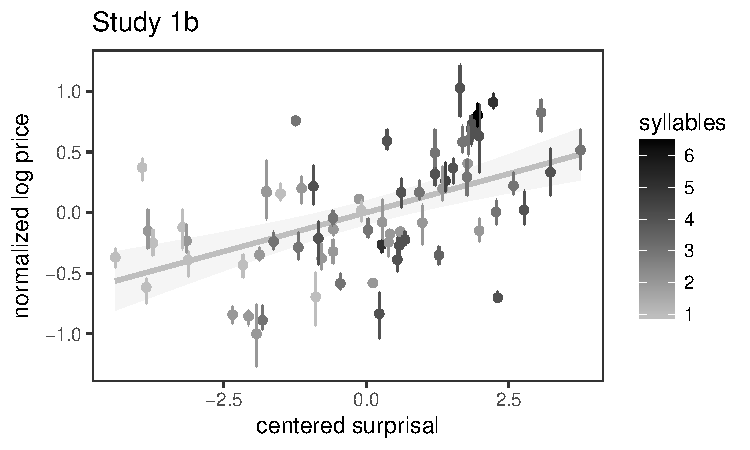
\includegraphics[width=0.5\textwidth]{images/plot_study1b.pdf}
\end{center}
\caption{Results of Study \hyperref[sec:study1b]{1b}. As surprisal increases, participants' scaled free response prices increase.} 
\label{fig:plot_study1b}
\end{figure}

\subsection{Study 2 \label{sec:study2}}

For Study \hyperref[sec:study2]{2} we used a forced-ranking dependent measure, which provides a more sensitive measure of the differences in degrees between similar adjective phrases.
This sensitivity makes Study \hyperref[sec:study2]{2} a better test of the independent effects of length and surprisal.
This depenent measure, because it does not depend on a numeric scale, also allows us to consider additional adjectival scales.

The M-implicature account described above implies that there is no semantic interaction between the intensifier and the adjective it is applied to.
Instead an intensifier should contribute similar cost, and therefore meaning, to the different adjective phrases in which it occurs\footnote{If the bigram frequency of the modified adjective phrase (\w{very expensive}) deviated from that expected based on independent word frequencies our frequency-based cost account would predict an interactive effect on meaning.
This would likely be a relatively small effect, and the relevant bigrams were too sparse in our corpora to pursue.}.
To explore this, we extend our results to four additional adjectival scales.


\subsubsection{Methods}

\paragraph{Participants}

30 participants with US IP addresses were recruited through Amazon's Mechanical Turk and paid \$0.40 for  participation. 2 participants were excluded from the analysis for admitting that they did not think they followed the instructions in a post-experiment survey.

\paragraph{Items}

The full set of intensifiers in Study \hyperref[sec:study2]{2} is identical to that of Study \hyperref[sec:study1a]{1a}. 
For Study \hyperref[sec:study2]{2}, we used a ranking dependent measure: asking participants to sort a set of adjective phrases according to strength.
Because arranging these phrases required participants to be aware of the full set of adjective phrases and access all of them on the same computer screen (which might vary in size for different participants), not all of our 40 intensifiers could effectively be presented at once.
To make the task easier for participants and to extend to more adjective scales, we divided the full set of intensifiers into 4 smaller sets, maintaining a range of syllable lengths and surprisal across the intensifiers in each smaller set.

With the ranking dependent measure, we no longer need the adjectives to correspond to a standard numeric scale.
We therefore included 4 adjectives: \w{old}, \w{expensive}, \w{beautiful}, and \w{tall}.

\paragraph{Procedure%
% \footnote{A demo of Study \hyperref[sec:study2]{2} can be found at \url{http://cocolab.stanford.edu/links_for_papers/bennett2017extremely/experiments/Study2/.}}}
% \footnote{
% Demos for all studies can be found at
% \url{http://cocolab.stanford.edu/links_for_papers/bennett2017extremely/demos/}
% }
}

\begin{figure}[hbt]
\begin{center}
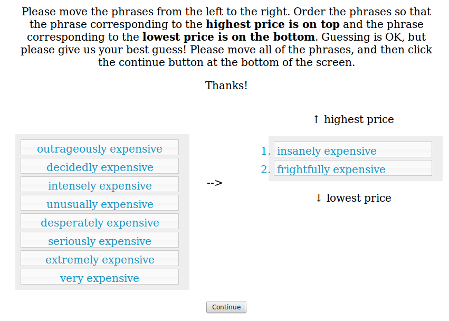
\includegraphics[width=0.4\textwidth]{exp2-q.png}
\end{center}
\caption{Screenshot from Study 2 target question.} 
\label{fig:question_study2}
\end{figure}

For each trial of Study \hyperref[sec:study2]{2}, we asked participants to order a set of 10 adjective phrases according to strength of meaning.
Adjective phrases were randomly ordered in a list on the left.
Participants were asked to move the adjective phrases from the left to the right side of the screen, reordering the phrases from the ``lowest'' to the ``highest'' degree (Figure~\hyperref[fig:question_study2]{\ref{fig:question_study2}}).
Each adjective phrase in a trial contained the same adjective, modified with different intensifiers.
Each participant saw 4 intensifier sets, each paired with one of the four adjectives.
The pairings of intensifier-sets to adjectives varied between participants.
Participants completed 4 such trials, ranking intensifiers for all 4 adjectives and all 4 intensifier sets.

\subsubsection{Analysis}

We ran a rank-ordered logit model \cite{beggs_assessing_1981, hausman_specifying_1987} with alternative-specific variables for surprisal and for length in syllables. This model did not include an intercept.
%
To test whether we find an interaction between intensifier strength and the adjective it modifies, we ran a second rank-ordered logit model with additional alternative-specific variables for the interaction between the adjective being modified and both surprisal and length. 

\subsubsection{Results}

Our results for Study 2 are shown in Figure~\ref{fig:plot_study2}\eb{, with full output in Appendix D}. In our first model, with surprisal and length as the only predictors in question, we again found a significant effect of surprisal ($b=0.164,t=10.128,p<0.0005$). We also find a significant effect of syllable length ($b=0.243,t=5.888,p<0.0005$).

In likelihood ratio tests, we again found that length alone accounts for the data less well than the full model ($\chi^2(1)=108.085, p<0.0005$) and that surprisal alone also accounts for the data less well than the full model ($\chi^2(1)=34.694, p<0.0005$).
When residualizing length with respect to surprisal, we again found a significant effect of surprisal ($b=0.19,t=11.663,p<0.0005$). In addition, with this more sensitive ranking measure, we found a significant effect of length residuals ($b=0.243,t=5.888,p<0.0005$).
When residualizing surprisal with respect to length, we found significant effects of length ($b=0.35,t=8.459,p<0.0005$) and surprisal residuals ($b=0.164,t=10.128,p<0.0005$).

In the second model, with adjective interactions, we again found significant effects of surprisal ($b=0.074, t=2.482, p=0.0131$) and length ($b=0.318, t=3.658, p=0.0003$), and also found a significant interaction between surprisal and the adjective being modified (estimates for \w{tall} and \w{expensive} were higher than for \w{beautiful}, while \w{old} was not significantly different from \w{beautiful}).
This suggests that context-specific surprisal (e.g.~bigram frequencies) might affect the utterance cost, or that factors of utterance cost might have different effects for different adjectives.

In other words, we again found that participants assign stronger interpretations to intensifiers with higher surprisals and/or higher syllable lengths, extending now across four different adjectival scales.
In addition, we found interactions between modifier and adjective (or perhaps scale).

\begin{figure*}[hbt]
\begin{center}
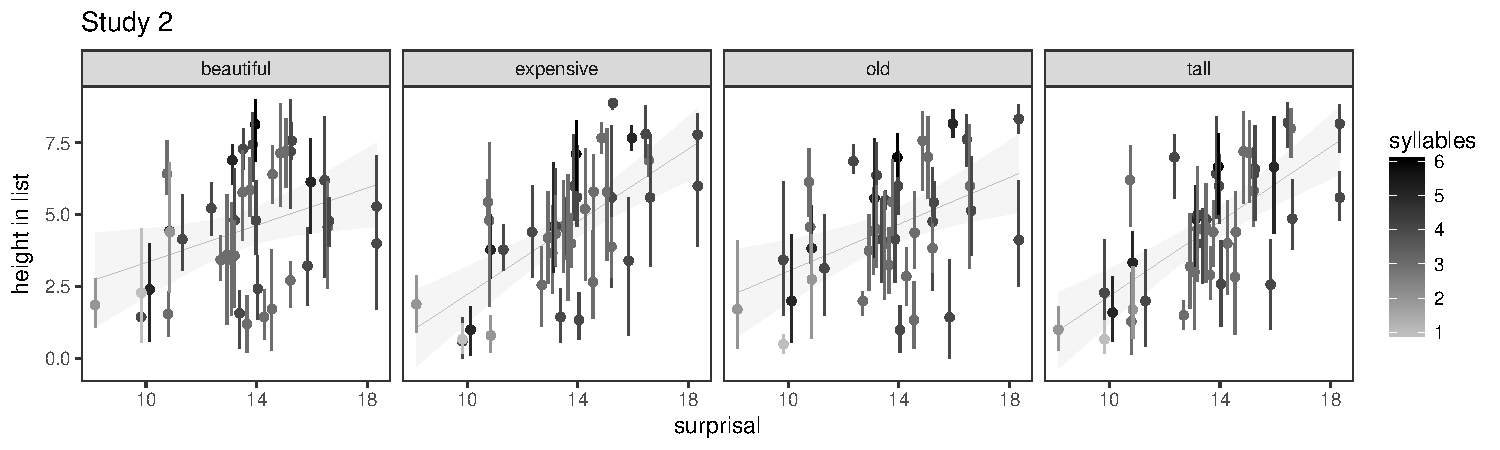
\includegraphics[width=\textwidth]{images/plot_study2.pdf}
\end{center}
\caption{Results of Study 2. As surprisal and length in syllables increase, participants' rankings increased.} 
\label{fig:plot_study2}
\end{figure*}

\subsection{Discussion}

In Studies 1a and 1b, we found evidence that an intensifier's surprisal is a significant predictor of strength of its meaning. In Study 2, we used a more sensitive dependent measure and showed that length in syllables is also a significant predictor of strength of meaning.
These studies taken together provide evidence that intensifier meanings depend systematically on the length and frequency of their word forms.

Since this is a correlational study, such a relationship does not confirm that an intensifier's cost \emph{causes} it to have a given meaning.

In particular, we can explain the correlation with rarity if the strength of an intensifier's meaning causes it to be rarely used.
That is, more extreme intensifiers naturally refer to less probable events and properties in the world, and therefore might be used less frequently\footnote{
However, note that the frequency with which things occur in the world does not map directly on to how often those things are talked about. 
Although it seems reasonable to suspect that word frequencies reflect the probabilities of the real-world concepts they describe, it might also be the case that improbable things are more likely to be commented on, and so to a certain extent the frequencies of words that describe rare concepts will be inflated. 
}.
Syllable length in turn can depend on the frequency, simplicity, or predictability of a word \cite{zipf_psycho-biology_1935, lewis_conceptual_2016, mahowald_info/information_2013}, either because words that are frequently used get shortened over time \cite{kanwal_evolution_2016} or perhaps because words that refer to simpler or more common concepts enter the lexicon sooner (when more short word forms remain to be assigned meanings).
It is therefore possible that neither of these measures of cost have causal influence on the meanings of intensifiers within a particular communicative act.

To more directly address the question of whether utterance cost \emph{causes} people to interpret an intensifier as stronger, we ran Studies 3 and 4, where we directly manipulated one of our measures of cost---length---in novel intensifiers which have no conventional meaning associated to them. 


\renewcommand{\baselinestretch}{0.7}


\begin{table}[hbt]
 \begin{center}
 \footnotesize
  \caption{Intensifiers from Study \hyperref[sec:study1a]{1a}, number of occurences in Google Web 1T 5grams corpus, and length in syllables.}
  \label{table:intensifiers_study1a}
  \begin{tabular}{lrc}
   \hline
   ngram & frequency & length \\
    \hline
    surpassingly & 11156 & 4 \\
    colossally & 11167 & 4 \\
    terrifically & 62292 & 4 \\
    frightfully & 65389 & 3 \\
    astoundingly & 73041 & 4 \\
    phenomenally & 120769 & 5 \\
    uncommonly & 135747 & 4 \\
    outrageously & 240010 & 4 \\
    fantastically & 250989 & 4 \\
    mightily & 252135 & 3 \\
    supremely & 296134 & 3 \\
    insanely & 359644 & 3 \\
    strikingly & 480417 & 3 \\
    acutely & 493931 & 3 \\
    awfully & 651519 & 3 \\
    decidedly & 817806 & 4 \\
    excessively & 877280 & 4 \\
    extraordinarily & 900456 & 6 \\
    exceedingly & 977435 & 4 \\
    intensely & 1084765 & 3 \\
    markedly & 1213704 & 3 \\
    amazingly & 1384225 & 4 \\
    radically & 1414254 & 3 \\
    unusually & 1583939 & 4 \\
    remarkably & 1902493 & 4 \\
    terribly & 1906059 & 3 \\
    exceptionally & 2054231 & 5 \\
    desperately & 2139968 & 3 \\
    utterly & 2507480 & 3 \\
    notably & 3141835 & 3 \\
    incredibly & 4416030 & 4 \\
    seriously & 12570333 & 4 \\
    truly & 19778608 & 2 \\
    significantly & 19939125 & 5 \\
    totally & 20950052 & 3 \\
    extremely & 21862963 & 3 \\
    particularly & 41066217 & 5 \\
    quite & 55269390 & 1 \\
    especially & 55397873 & 4 \\
    very & 292897993 & 2 \\
   \hline
  \end{tabular}
 \end{center}
\end{table}



\begin{table}[hbt]
 \begin{center}
 \footnotesize
  \caption{Intensifiers from Study1b, number of occurences in Google Web 1T 5grams corpus, and length in syllables.}
  \label{table:intensifiers_study1b}
  \begin{tabular}{lrc}
   \hline
   intensifier & freq & syll \\
   \hline
    dreadfully & 147917 & 3 \\ 
    fantastically & 250989 & 4 \\ 
    supremely & 296134 & 3 \\ 
    suspiciously & 398581 & 4 \\ 
    strikingly & 480417 & 3 \\ 
    noticeably & 632679 & 4 \\ 
    awfully & 651519 & 3 \\ 
    unbelievably & 686210 & 5 \\ 
    downright & 876782 & 2 \\ 
    excessively & 877280 & 4 \\ 
    extraordinarily & 900456 & 6 \\ 
    exceedingly & 977435 & 4 \\ 
    tremendously & 989532 & 4 \\ 
    enormously & 1011751 & 4 \\ 
    immensely & 1061341 & 3 \\ 
    hugely & 1074430 & 2 \\ 
    intensely & 1084765 & 3 \\ 
    profoundly & 1172521 & 3 \\ 
    infinitely & 1226005 & 4 \\ 
    amazingly & 1384225 & 4 \\ 
    unusually & 1583939 & 4 \\ 
    outright & 1662351 & 2 \\ 
    wonderfully & 1776763 & 3 \\ 
    remarkably & 1902493 & 4 \\ 
    terribly & 1906059 & 3 \\ 
    sharply & 2377367 & 2 \\ 
    utterly & 2507480 & 3 \\ 
    positively & 3225521 & 4 \\ 
    extensively & 3447083 & 4 \\ 
    mighty & 3492518 & 2 \\ 
    surprisingly & 3554188 & 4 \\ 
    altogether & 3683374 & 4 \\ 
    purely & 4201779 & 2 \\ 
    wholly & 4308225 & 2 \\ 
    incredibly & 4416030 & 4 \\ 
    badly & 4808245 & 2 \\ 
    considerably & 4834700 & 5 \\ 
    sufficiently & 5059075 & 4 \\ 
    good and & 5671809 & 2 \\ 
    thoroughly & 6167601 & 3 \\ 
    damn & 6930185 & 1 \\ 
    deeply & 7242890 & 2 \\ 
    perfectly & 10031907 & 3 \\ 
    greatly & 11337773 & 2 \\ 
    largely & 11379702 & 2 \\ 
    very much & 11415215 & 3 \\ 
    strongly & 13931652 & 2 \\ 
    entirely & 14720396 & 4 \\ 
    plain & 15433319 & 1 \\ 
    absolutely & 16064235 & 4 \\ 
    truly & 19778608 & 2 \\ 
    totally & 20950052 & 3 \\ 
    extremely & 21862963 & 3 \\ 
    dead & 28609410 & 1 \\ 
    completely & 32310795 & 3 \\ 
    highly & 36460329 & 2 \\ 
    extra & 36838459 & 2 \\ 
    easily & 39241261 & 3 \\ 
    fully & 41415591 & 2 \\ 
    pretty & 43623658 & 2 \\ 
    simply & 50172762 & 2 \\ 
    quite & 55269390 & 1 \\ 
    rather & 66341863 & 2 \\ 
    real & 144660526 & 1 \\ 
    really & 148918637 & 2 \\ 
    too & 159399185 & 1 \\ 
    way & 268084494 & 1 \\ 
    very & 292897993 & 2 \\ 
    well & 301853777 & 1 \\ 
    most & 324420476 & 1 \\ 
    so & 518878130 & 1 \\
   \hline
  \end{tabular}
 \end{center}
\end{table}

\renewcommand{\baselinestretch}{1.0}